\documentclass{standalone}
\usepackage{tikz}
\usetikzlibrary{positioning}

\begin{document}
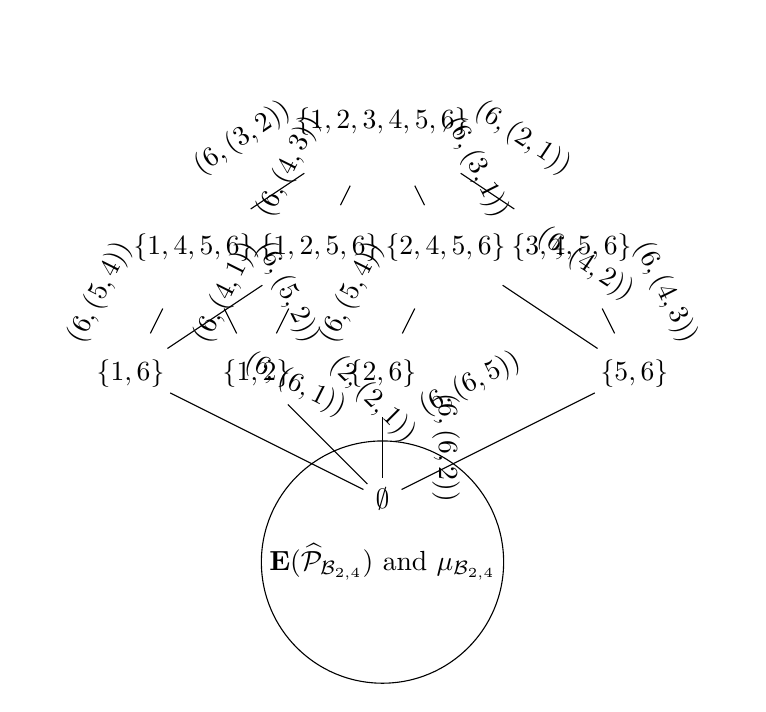
\begin{tikzpicture}[scale=0.8, every node/.style={circle, inner sep=2pt}]
    % Nodes
    \node (max) at (0,4) {$\{1,2,3,4,5,6\}$};
    \node (a) at (-3,2) {$\{1,4,5,6\}$};
    \node (b) at (-1,2) {$\{1,2,5,6\}$};
    \node (c) at (1,2) {$\{2,4,5,6\}$};
    \node (d) at (3,2) {$\{3,4,5,6\}$};
    \node (a1) at (-4,0) {$\{1,6\}$};
    \node (a2) at (-2,0) {$\{1,2\}$};
    \node (a3) at (0,0) {$\{2,6\}$};
    \node (a4) at (4,0) {$\{5,6\}$};
    \node (min) at (0,-2) {$\emptyset$};

    % Edges
    \draw (max) -- (a) node[midway, sloped, above] {$(6,(3,2))$};
    \draw (max) -- (b) node[midway, sloped, above] {$(6,(4,3))$};
    \draw (max) -- (c) node[midway, sloped, above] {$(6,(3,1))$};
    \draw (max) -- (d) node[midway, sloped, above] {$(6,(2,1))$};
    
    \draw (a) -- (a1) node[midway, sloped, above] {$(6,(5,4))$};
    \draw (a) -- (a2) node[midway, sloped, above] {$(6,(5,2))$};
    \draw (b) -- (a1) node[midway, sloped, above] {}; % Remove or adjust label if not needed
    \draw (b) -- (a2) node[midway, sloped, above] {$(6,(4,1))$};
    \draw (c) -- (a3) node[midway, sloped, above] {$(6,(5,4))$};
    \draw (c) -- (a4) node[midway, sloped, above] {$(6,(4,2))$};
    \draw (d) -- (a4) node[midway, sloped, above] {$(6,(4,3))$};
    
    \draw (a1) -- (min) node[midway, sloped, above] {$(6,(6,1))$};
    \draw (a2) -- (min) node[midway, sloped, above] {$(2,(2,1))$};
    \draw (a3) -- (min) node[midway, sloped, above] {$(6,(6,2))$};
    \draw (a4) -- (min) node[midway, sloped, above] {$(6,(6,5))$};
    
    % Additional annotations as per the description
    \node[draw, align=left] at (0,-3) {$\mathbf{E}(\widehat{\mathcal{P}}_{\mathcal{B}_{2,4}})$ and $\mu_{\mathcal{B}_{2,4}}$};
\end{tikzpicture}
\end{document}